\documentclass[12pt]{article}

\usepackage{bm}
\usepackage{amsmath}
\usepackage{amssymb}
\usepackage{cite}
\usepackage{indentfirst}
\usepackage{url}
\usepackage{graphicx}

\title{Project 1 \\\vspace{1em}
\large CS 525: Deep Learning}
\author{
  Jerry Duncan \\
  jdunca51@vols.utk.edu
}
\date{January 30, 2019}
\begin{document}
\maketitle
\pagebreak

\section{Introduction}

For this project, we're trying to create a Neural Network library that is both functional and extensible in the future.
Specifically to be extended to Convolutional Neural Networks.
Neural Networks are able to solve a large range of problems and are paramount to success in today's data driven world.
In order to better understand how they work, it's our job to completely program one from scratch with only Numpy at our disposal.
Once completed, we should be able to train it to solve a variety of problems, but for this specific project, we'll just be tasking it with correctly predicting AND and XOR.

\section{Assumptions / Choices Made}

To simplify the training of the network, I've made the following choices.
\begin{itemize}
  \item My calculateloss method takes in an array of inputs and outputs and returns the weighted loss
  \item My train method takes in an array of inputs and outputs and trains on the whole set for a specified number of epochs
\end{itemize}

To add additional features and simplify other parts of the code, I've made the following choices.
\begin{itemize}
  \item I import pickle to conveniently save and load models and model weights
  \item I import abspath and isfile from os.path to help with error checking files before saving/loading models and model weights
\end{itemize}

\section{Problems / Issues}

Nothing to add.

\section{Running My Code}

The only differences from the stated requirements and my code is as follows:
\begin{itemize}
  \item My calculateloss method takes in an array of inputs and outputs and returns the weighted loss
  \item My train method takes in an array of inputs and outputs and trains on the whole set for a specified number of epochs
\end{itemize}

\section{Graphs}

\subsection{AND}
Typically learning rates are between 0 and 1.
In order to find a learning rate that is clearly too high, however, I had to increase it above 1.
As we can see in Figure \ref{fig:and10}, it takes a learning rate of 50 for the network to learn AND so poorly.
In Figure \ref{fig:and10000}, we can actually see that even a learning rate of 100 was able to get lucky and find a set of correct weights as it was able to learn AND after about 3750 epochs.
As for a learning rate that's too low, we can look at Figure \ref{fig:and1000} to see that the majority of the networks that managed to learn AND did so in around 200 epochs.
Using that as the qualifying factor, it would seem that a learning rate lower than 0.5 is too low to efficiently learn AND.
If we look at how they all fared over 10,000 epochs in Figure \ref{fig:and10000}, we can see that the only network that was really too slow was the one with a learning rate of 0.01.
So, for AND, we can experimentally conclude that a learning rate of 0.05 to 1 is ideal.

\subsection{XOR}

For XOR, the story is a little different.
It takes all of the networks a considerable amount of time to learn XOR, regardless of learning rate.
Again, we take a look at learning rates above 1 to see what it takes for a learning rate to truly be too high.
If we look at Figure \ref{fig:xor100}, we can see that a learning rate of 5 managed to luckily learn XOR, but this should be taken with a grain of salt as this is not the norm.
When we look at a 1,000 epochs in Figure \ref{fig:xor1000}, we can see that 0.5 learns XOR the fastest (disregarding 5).
And when we extend that to 10,000 in Figure \ref{fig:xor10000}, we can see that any learning rate between 0.05 and 0.5 is able to eventually learn XOR.
So, for XOR, we can experimentally conclude that a learning rate of 0.05 to 0.5 is able to learn XOR, but a learning rate of 0.5 is likely ideal.

\subsection{Conclusions}

It's important to clarify that the conclusions just made are experimental and only run with a single seed.
In order to get a better idea of what learning rate is best for these problems, we would need numerous network initializations over each learning rate to get the full picture.

\begin{figure}[!htb]
  \centering
  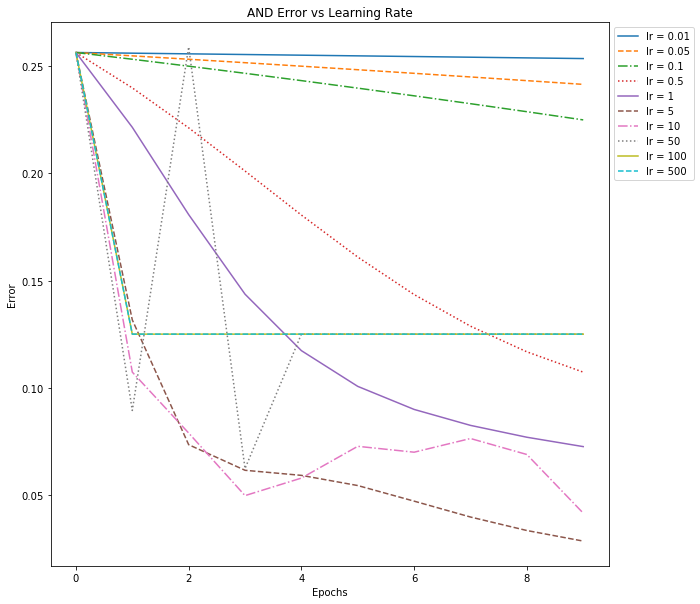
\includegraphics[width=\linewidth]{and_10.png}
  \caption{Learning rates on AND over 10 epochs.}
  \label{fig:and10}
\end{figure}

\begin{figure}
  \centering
  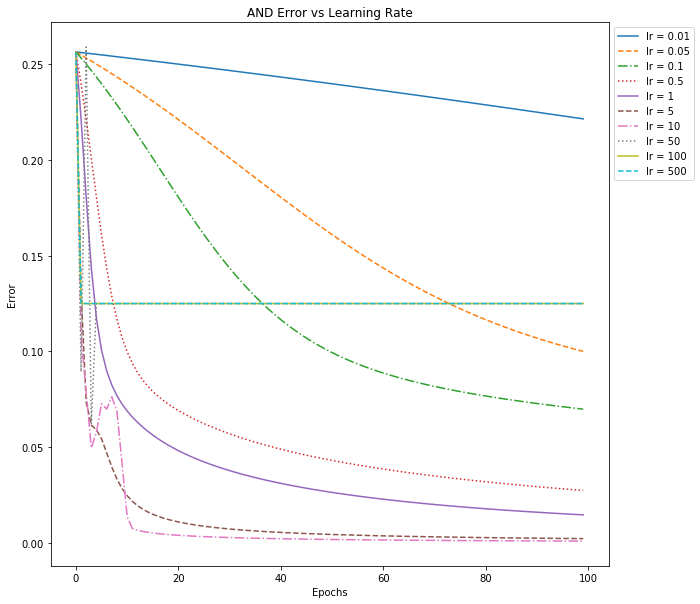
\includegraphics[width=\linewidth]{and_100.png}
  \caption{Learning rates on AND over 100 epochs.}
  \label{fig:and100}
\end{figure}

\begin{figure}
  \centering
  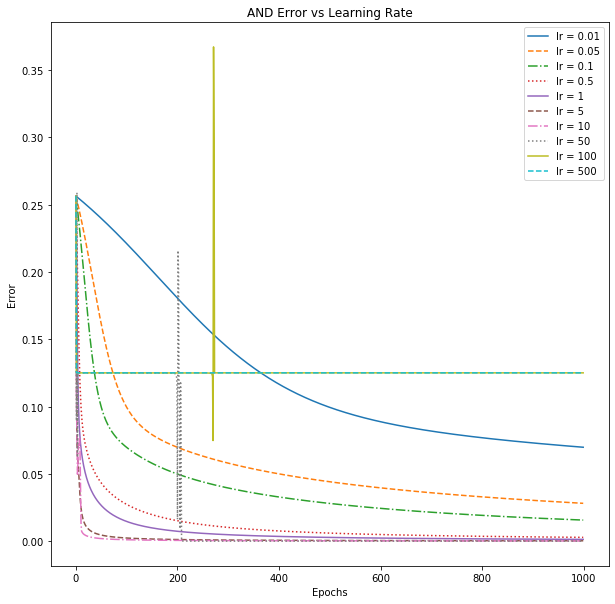
\includegraphics[width=\linewidth]{and_1000.png}
  \caption{Learning rates on AND over 1000 epochs.}
  \label{fig:and1000}
\end{figure}

\begin{figure}
  \centering
  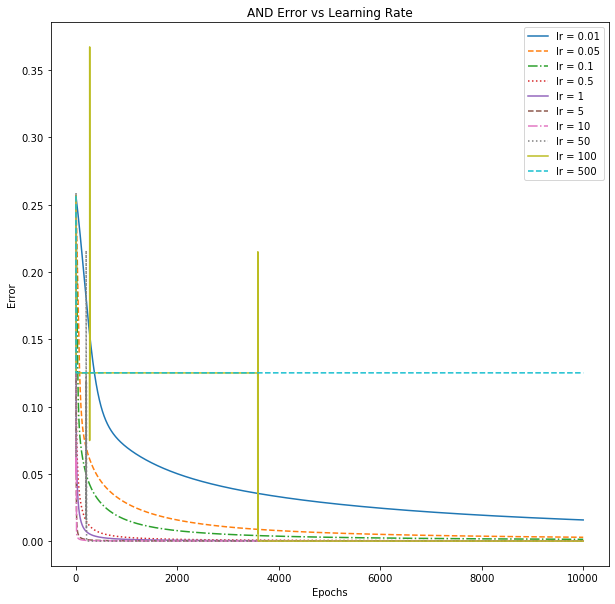
\includegraphics[width=\linewidth]{and_10000.png}
  \caption{Learning rates on AND over 10000 epochs.}
  \label{fig:and10000}
\end{figure}

\begin{figure}
  \centering
  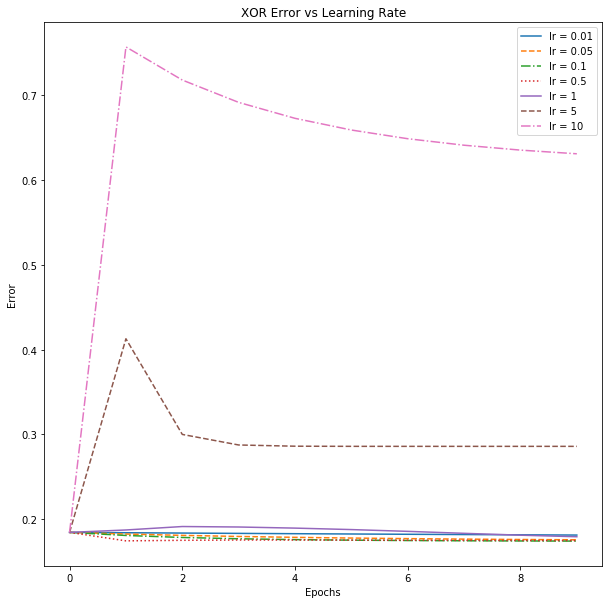
\includegraphics[width=\linewidth]{xor_10.png}
  \caption{Learning rates on XOR over 10 epochs.}
  \label{fig:xor10}
\end{figure}

\begin{figure}
  \centering
  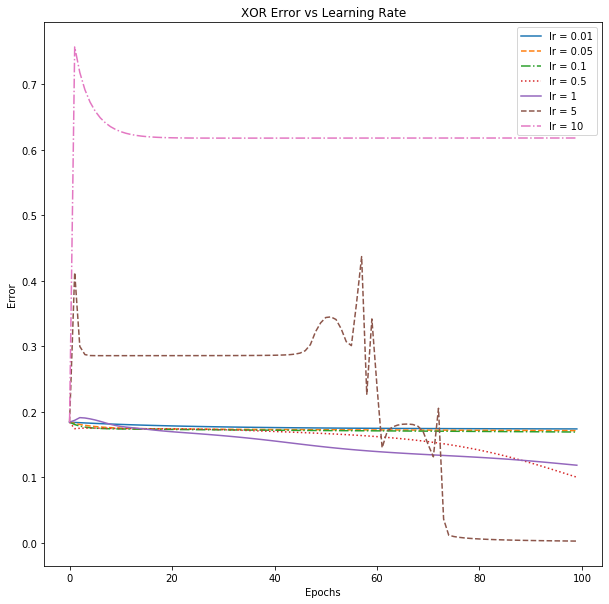
\includegraphics[width=\linewidth]{xor_100.png}
  \caption{Learning rates on XOR over 100 epochs.}
  \label{fig:xor100}
\end{figure}

\begin{figure}
  \centering
  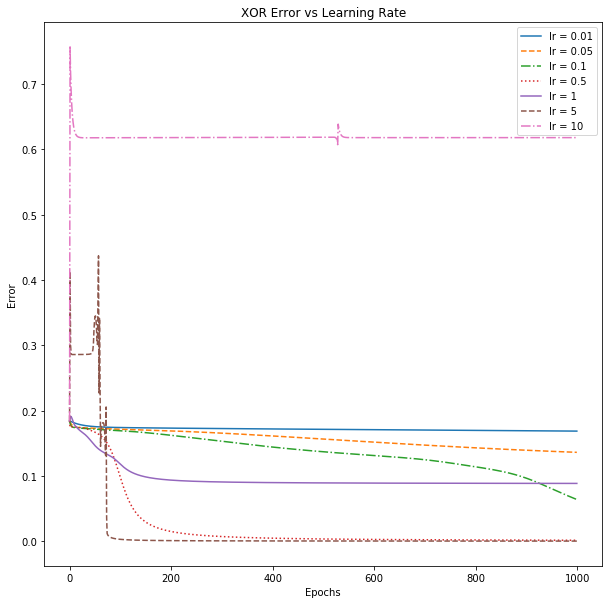
\includegraphics[width=\linewidth]{xor_1000.png}
  \caption{Learning rates on XOR over 1000 epochs.}
  \label{fig:xor1000}
\end{figure}

\begin{figure}
  \centering
  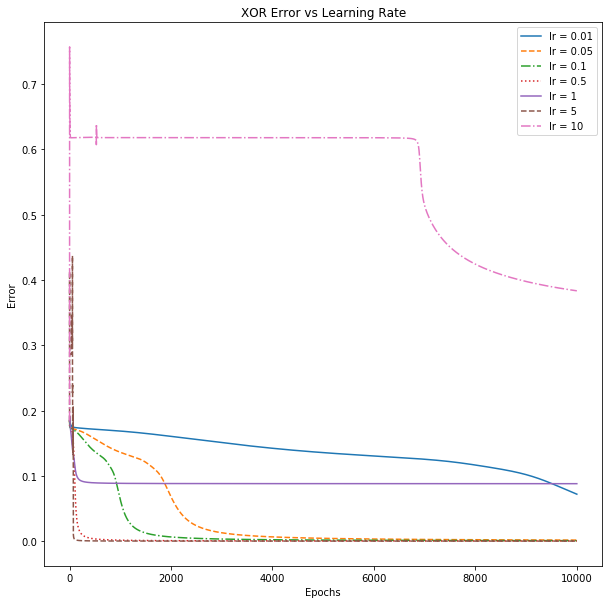
\includegraphics[width=\linewidth]{xor_10000.png}
  \caption{Learning rates on XOR over 10000 epochs.}
  \label{fig:xor10000}
\end{figure}

\bibliographystyle{abbrv}

\end{document}